\section{Auswertung}
    \subsection{Ätzgrübchendichte}
        Zunächst gilt es die Nominale Unordnung der Proben zu definieren, dies lässt sich über die Ätzgrübchendichte an der Oberfläche
        realisieren. Dazu wurden für beide Proben je 3 Bilder von verschiedenen Positionen an der Oberfläche aufgenommen und anschließend
        aus der Fläche, aufgenommen durch das Mikroskop, und den sichtbaren Ätzgrübchen die Ätzgrübchendichte bestimmt. Dieser Vorgang ist,
        durch das manuelle Zählen der Grübchen sehr müßig und ungenau, lässt aber dennoch eine Qualitative aussage über die Ordnung im Kristall zu.
        Aus den Aufgenommen Bildern lies sich folgende Tabelle erstellen.
        \begin{table}[H]
            \centering
            \begin{tabular}[]{c|c|c|c|c}
                Probe & Aufnahme Nr. & Anzahl Grübchen & Fläche [$\mu m^2$] & Dichte [$\frac{n}{\mu m^2}$] \\
                \hline
                \multirow{3}{*}{\rotatebox[origin=c]{90}{Get.}} & 1 & $39 \pm 3$ & 839908,67 & 4,64e-5 \\
                                                                     & 2 & $25 \pm 3$ & 1099357,61& 2,27e-5 \\
                                                                     & 3 & $31 \pm 3$ & 454314,66 & 6,82e-5 \\
                Mittelwert                                           & - & - & - & $4,58e-5 \pm 2,27$\\
                \hline
                \multirow{3}{*}{\rotatebox[origin=c]{90}{Unget.}}  & 1 & $344 \pm 40$  & 18894,73 & 0,018 \\
                                                                        & 2 & $27 \pm 5$    & 7942,73 & 0,003 \\
                                                                        & 3 & $103 \pm 15$  & 6251,25 & 0,017 \\
                Mittelwert                                           & - & - & - & $0,013 \pm 0,008$\\
                
            \end{tabular}    
        \end{table}
        Es ist deutlich zu erkennen, dass die Ätzgrübchendichte der ungetemperten Probe um ein Vielfaches höher ist, als die der getemperten.
        Auch ist zu erkennen, dass die Ätzgrübchendichte an verschiedenen stellen der Oberfläche stark variiert, also nicht konstant ist.
    \begin{figure}[H]
        \centering
        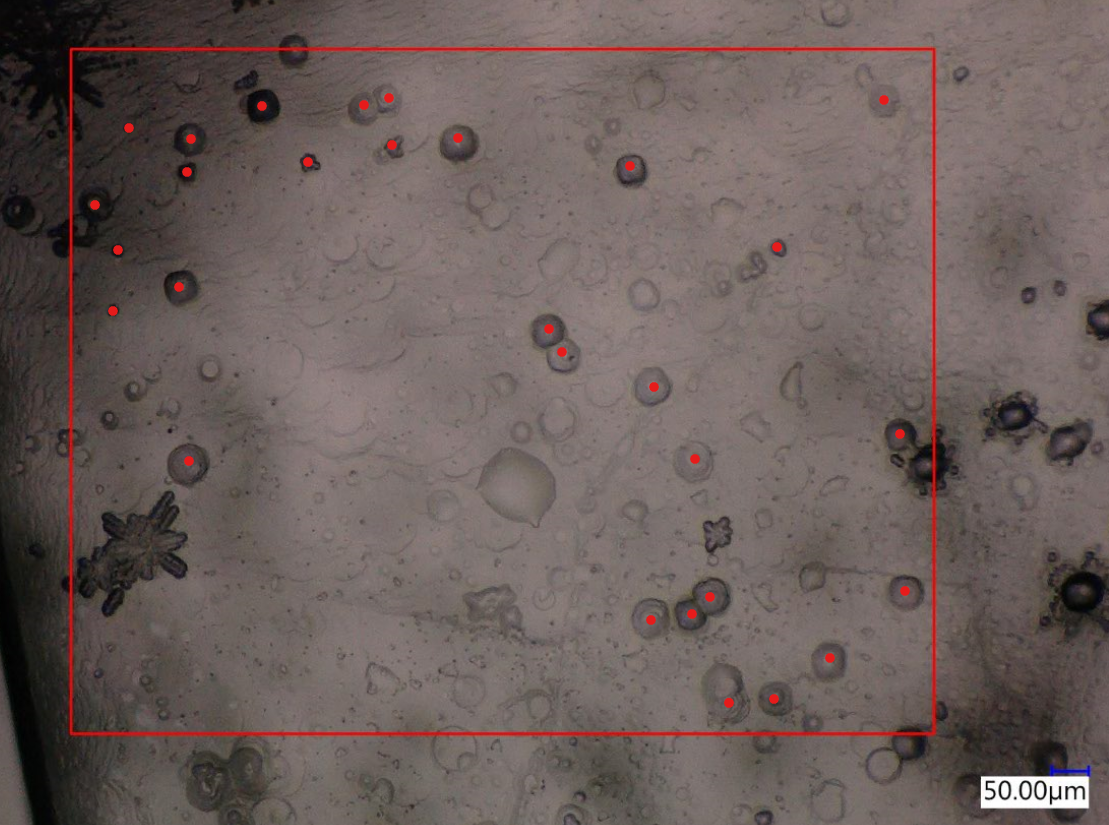
\includegraphics[width=\textwidth]{Images/Beispiel_ätzgrübchendichte.PNG}
        \caption{Beispiel einer Aufnahme für die Ätzgrübchendichte.}
    \end{figure}

